\newpage
\subsection{Caso d'uso UC10: Visualizzazione API registrate}
\label{UC10}
\begin{figure}[ht]
	\centering
	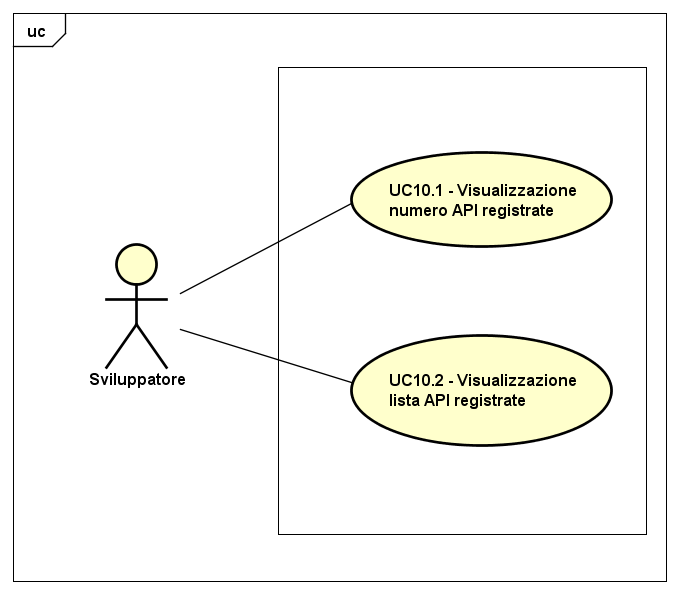
\includegraphics[scale=0.45]{UML/UC10.png}
	\caption{UC10: Visualizzazione API registrate}
\end{figure}

\begin{longtable}{ l | p{11cm}}
	\hline
	\rowcolor{Gray}
	\multicolumn{2}{c}{UC10 - Visualizzazione API registrate}\\
	\hline
	\textbf{Attori} & Sviluppatore \\
	\textbf{Descrizione} & L'attore visualizza le API da lui registrate \\
	\textbf{Pre-Condizioni} & L'attore si trova nella schermata relativa alle API da lui registrate \\
	\textbf{Post-Condizioni} & L'attore ha visualizzato le API da lui registrate \\
	\textbf{Scenario Principale} & 
	\begin{enumerate*}[label=(\arabic*.),itemjoin={\newline}]
		\item L'attore può visualizzare il numero delle API da lui registrate (UC10.1)
		\item L'attore può visualizzare la lista delle API da lui registrate (UC10.2)
	\end{enumerate*}\\
\end{longtable}

\subsubsection{Caso d'uso UC10.1: Visualizzazione numero API registrate}
\label{UC10_1}

\begin{minipage}{\linewidth}
	\begin{tabular}{ l | p{11cm}}
		\hline
		\rowcolor{Gray}
		\multicolumn{2}{c}{UC10.1 - Visualizzazione numero API registrate} \\
		\hline
		\textbf{Attori} & Sviluppatore \\
		\textbf{Descrizione} & L'attore visualizza il numero di API da lui registrate \\
		\textbf{Pre-Condizioni} & L'attore si trova nella schermata relativa alle API da lui registrate \\
		\textbf{Post-Condizioni} & L'attore ha visualizzato il numero delle API da lui registrate \\
		\textbf{Scenario Principale} & 
		\begin{enumerate*}[label=(\arabic*.),itemjoin={\newline}]
			\item L'attore può visualizzare il numero di API da lui registrate
		\end{enumerate*}\\
	\end{tabular}
\end{minipage}

\newpage
\subsubsection{Caso d'uso UC10.2: Visualizzazione lista API registrate}
\label{UC10_2}
\begin{figure}[ht]
	\centering
	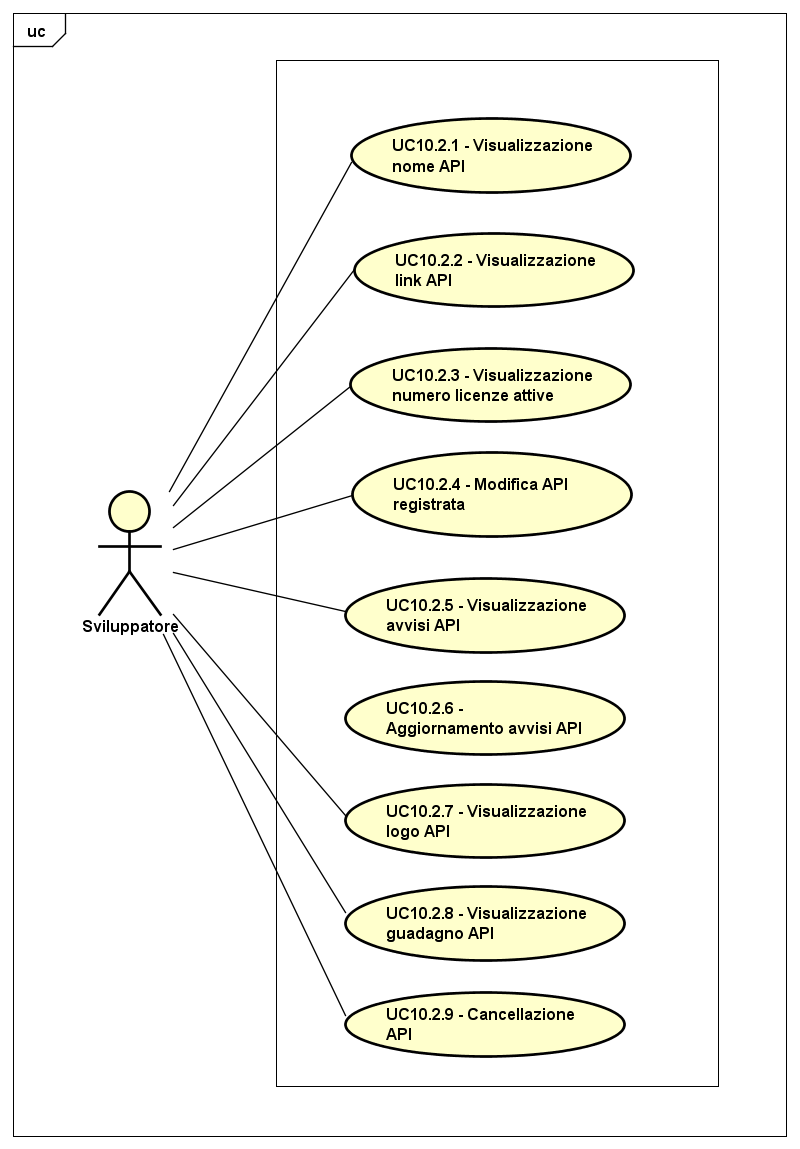
\includegraphics[scale=0.45]{UML/UC10_2.png}
	\caption{UC10.2: Visualizzazione lista API registrate}
\end{figure}

\begin{minipage}{\linewidth}
	\begin{tabular}{ l | p{11cm}}
		\hline
		\rowcolor{Gray}
		\multicolumn{2}{c}{UC10.2 - Visualizzazione lista API registrate} \\
		\hline
		\textbf{Attori} & Sviluppatore \\
		\textbf{Descrizione} & L'attore visualizza la lista delle API da lui registrata \\
		\textbf{Pre-Condizioni} & L'attore si trova nella schermata relativa alle API da lui registrate \\
		\textbf{Post-Condizioni} & L'attore ha visualizzato la lista delle API da lui registrate \\
		\textbf{Scenario Principale} & 
		\begin{enumerate*}[label=(\arabic*.),itemjoin={\newline}]
			\item L'attore può visualizzare il nome dell'API (UC10.2.1)
			\item L'attore può visualizzare il link alla pagina di visualizzazione API (UC10.2.2)
			\item L'attore può visualizzare il numero di licenze attive dell'API (UC10.2.3)
			\item L'attore può modificare l'API (UC10.2.4)
			\item L'attore può visualizzare gli avvisi riguardo l'API (UC10.2.5)
			\item L'attore può aggiornare gli avvisi riguardo allo status dell'API (UC10.2.6)
			\item L'attore può visualizzare il logo dell'API (UC10.2.7)
			\item L'attore può visualizzare il guadagno dell'API (UC10.2.8)
		\end{enumerate*}\\
	\end{tabular}
\end{minipage}

\paragraph{Caso d'uso UC10.2.1: Visualizzazione nome API}
\label{UC10_2_1}

\begin{minipage}{\linewidth}
	\begin{tabular}{ l | p{11cm}}
		\hline
		\rowcolor{Gray}
		\multicolumn{2}{c}{UC10.2.1 - Visualizzazione nome API} \\
		\hline
		\textbf{Attori} & Sviluppatore \\
		\textbf{Descrizione} & L'attore visualizza nella lista il nome di ogni API da lui registrata \\
		\textbf{Pre-Condizioni} & L'attore si trova nella schermata relativa alle API da lui registrate \\
		\textbf{Post-Condizioni} & L'attore ha visualizzato nella lista il nome di ogni API da lui registrata \\
		\textbf{Scenario Principale} & 
		\begin{enumerate*}[label=(\arabic*.),itemjoin={\newline}]
			\item L'attore può visualizzare nella lista il nome di ogni API da lui registrata
		\end{enumerate*}\\
	\end{tabular}
\end{minipage}

\paragraph{Caso d'uso UC10.2.2: Visualizzazione link API}
\label{UC10_2_2}

\begin{minipage}{\linewidth}
	\begin{tabular}{ l | p{11cm}}
		\hline
		\rowcolor{Gray}
		\multicolumn{2}{c}{UC10.2.2 - Visualizzazione link API} \\
		\hline
		\textbf{Attori} & Sviluppatore \\
		\textbf{Descrizione} & L'attore visualizza nella lista il link alla visualizzazione dell'API  \\
		\textbf{Pre-Condizioni} & L'attore si trova nella schermata relativa alle API da lui registrate \\
		\textbf{Post-Condizioni} & L'attore ha visualizzato nella lista il link alla visualizzazione dell'API \\
		\textbf{Scenario Principale} & 
		\begin{enumerate*}[label=(\arabic*.),itemjoin={\newline}]
			\item L'attore può visualizzare nella lista il link alla visualizzazione dell'API, che lo reindirizzerà ad UC7 per l'API in questione
		\end{enumerate*}\\
	\end{tabular}
\end{minipage}

\paragraph{Caso d'uso UC10.2.3: Visualizzazione numero licenze attive}
\label{UC10_2_3}

\begin{minipage}{\linewidth}
	\begin{tabular}{ l | p{11cm}}
		\hline
		\rowcolor{Gray}
		\multicolumn{2}{c}{UC10.2.3 - Visualizzazione numero licenze attive} \\
		\hline
		\textbf{Attori} & Sviluppatore \\
		\textbf{Descrizione} & L'attore visualizza nella lista il numero di licenze attive per ogni API da lui registrata \\
		\textbf{Pre-Condizioni} & L'attore si trova nella schermata relativa alle API da lui registrate \\
		\textbf{Post-Condizioni} & L'attore ha visualizzato nella lista il numero di licenze attive per ogni API da lui registrata \\
		\textbf{Scenario Principale} & 
		\begin{enumerate*}[label=(\arabic*.),itemjoin={\newline}]
			\item L'attore può visualizzare nella lista il numero di licenze attive per ogni API da lui registrata
		\end{enumerate*}\\
	\end{tabular}
\end{minipage}

\newpage
\paragraph{Caso d'uso UC10.2.4: Modifica API registrata}
\label{UC10_2_4}
\begin{figure}[ht]
	\centering
	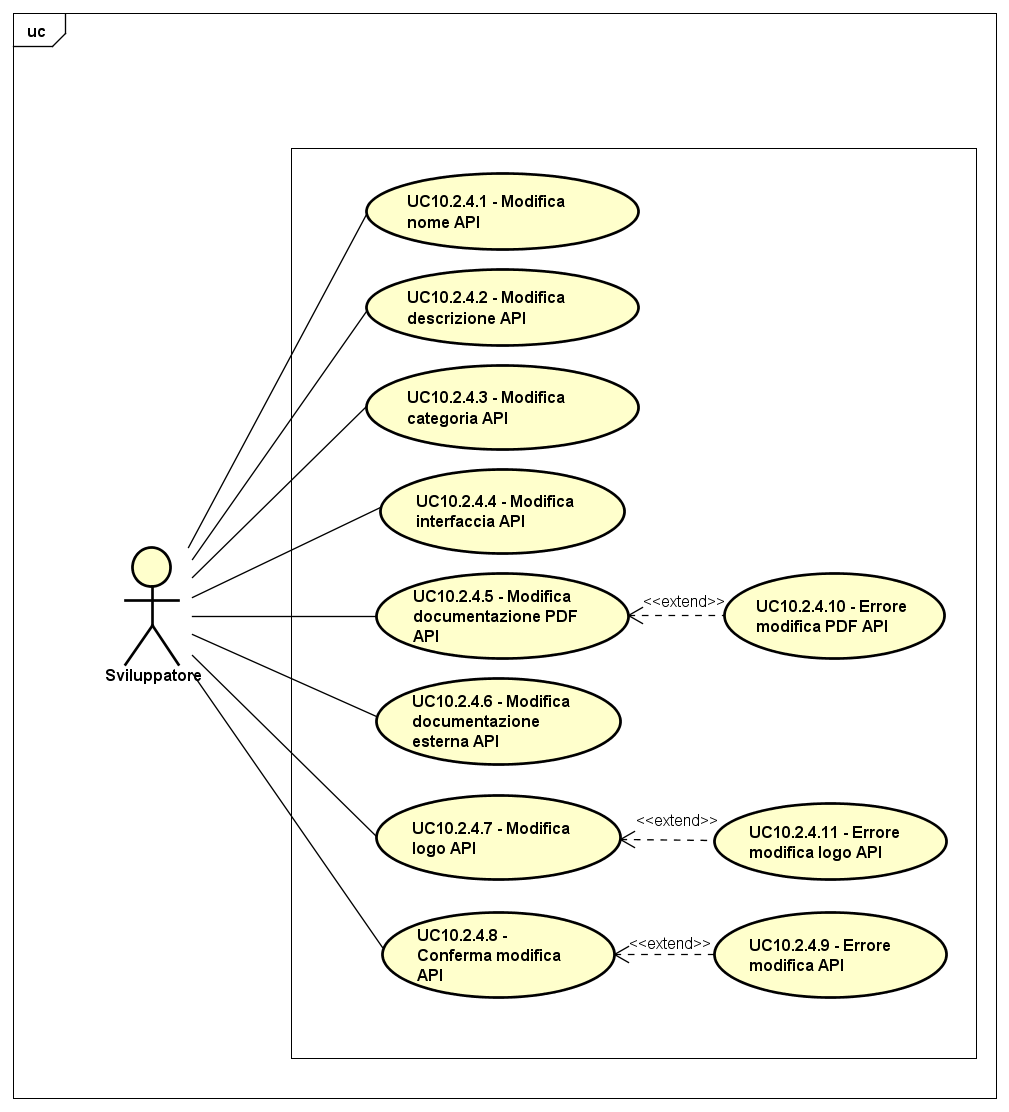
\includegraphics[scale=0.45]{UML/UC10_2_4.png}
	\caption{UC10.2.4: Modifica API registrata}
\end{figure}

\begin{minipage}{\linewidth}
	\begin{tabular}{ l | p{11cm}}
		\hline
		\rowcolor{Gray}
		\multicolumn{2}{c}{UC10.2.4 - Modifica API registrata} \\
		\hline
		\textbf{Attori} & Sviluppatore \\
		\textbf{Descrizione} & L'attore modifica una API da lui registrata \\
		\textbf{Pre-Condizioni} & L'attore si trova nella schermata relativa alle API da lui registrate \\
		\textbf{Post-Condizioni} & L'attore ha modificato un API registrata \\
		\textbf{Scenario Principale} & 
		\begin{enumerate*}[label=(\arabic*.),itemjoin={\newline}]
			\item L'attore può modificare il nome dell'API (UC10.2.4.1)
			\item L'attore può modificare la descrizione dell'API (UC10.2.4.2)
			\item L'attore può modificare la categoria dell'API (UC10.2.4.3)
			\item L'attore può modificare l'interfaccia dell'API (UC10.2.4.4)
			\item L'attore può modificare il file per la documentazione PDF (UC10.2.4.5)
			\item L'attore può modificare il link per la documentazione esterna (UC10.2.4.6)
			\item L'attore può modificare il logo dell'API (UC10.2.4.7)
			\item L'attore può confermare la modifica dell'API (UC10.2.4.8)
		\end{enumerate*}\\
		\textbf{Scenari Alternativi} & 
		\begin{enumerate*}[label=(\arabic*.),itemjoin={\newline}]
			\item L'attore può visualizzare un messaggio di errore riguardo al caricamento del file di documentazione PDF dell'API, ed il caricamento del file non avviene (UC10.2.4.10)
			\item L'attore può visualizzare un messaggio di errore riguardo al caricamento del file del logo dell'API, ed il caricamento del file non avviene (UC10.2.4.11)
			\item L'attore, dopo aver confermato le modifiche dell'API, può visualizzare un messaggio d'errore informativo e le modifiche non avvengono (UC10.2.4.9)
		\end{enumerate*}\\
	\end{tabular}
\end{minipage}

\subparagraph{Caso d'uso UC10.2.4.1: Modifica nome API}
\label{UC10_2_4_1}

\begin{minipage}{\linewidth}
	\begin{tabular}{ l | p{11cm}}
		\hline
		\rowcolor{Gray}
		\multicolumn{2}{c}{UC10.2.4.1 - Modifica nome API} \\
		\hline
		\textbf{Attori} & Sviluppatore \\
		\textbf{Descrizione} & L'attore modifica il nome dell'API \\
		\textbf{Pre-Condizioni} & L'attore si trova nella schermata relativa alla modifica di una API registrata, precedentemente selezionata \\
		\textbf{Post-Condizioni} & L'attore ha modificato il nome dell'API selezionata \\
		\textbf{Scenario Principale} & 
		\begin{enumerate*}[label=(\arabic*.),itemjoin={\newline}]
			\item L'attore può modificare il nome dell'API
		\end{enumerate*}\\
	\end{tabular}
\end{minipage}

\subparagraph{Caso d'uso UC10.2.4.2: Modifica descrizione API}
\label{UC10_2_4_2}

\begin{minipage}{\linewidth}
	\begin{tabular}{ l | p{11cm}}
		\hline
		\rowcolor{Gray}
		\multicolumn{2}{c}{UC10.2.4.2 - Modifica descrizione API} \\
		\hline
		\textbf{Attori} & Sviluppatore \\
		\textbf{Descrizione} & L'attore modifica la descrizione dell'API\\
		\textbf{Pre-Condizioni} & L'attore si trova nella schermata relativa alla modifica di una API registrata, precedentemente selezionata \\
		\textbf{Post-Condizioni} & L'attore ha modificato la descrizione dell'API selezionata \\
		\textbf{Scenario Principale} & 
		\begin{enumerate*}[label=(\arabic*.),itemjoin={\newline}]
			\item L'attore può modificare la descrizione dell'API
		\end{enumerate*}\\
	\end{tabular}
\end{minipage}

\subparagraph{Caso d'uso UC10.2.4.3: Modifica categoria API}
\label{UC10_2_4_3}

\begin{minipage}{\linewidth}
	\begin{tabular}{ l | p{11cm}}
		\hline
		\rowcolor{Gray}
		\multicolumn{2}{c}{UC10.2.4.3 - Modifica categoria API} \\
		\hline
		\textbf{Attori} & Sviluppatore \\
		\textbf{Descrizione} & L'attore modifica la categoria dell'API \\
		\textbf{Pre-Condizioni} & L'attore si trova nella schermata relativa alla modifica di una API registrata, precedentemente selezionata \\
		\textbf{Post-Condizioni} & L'attore ha modificato la categoria dell'API selezionata \\
		\textbf{Scenario Principale} & 
		\begin{enumerate*}[label=(\arabic*.),itemjoin={\newline}]
			\item L'attore può modificare la categoria dell'API
		\end{enumerate*}\\
	\end{tabular}
\end{minipage}

\subparagraph{Caso d'uso UC10.2.4.4: Modifica interfaccia API}
\label{UC10_2_4_4}

\begin{minipage}{\linewidth}
	\begin{tabular}{ l | p{11cm}}
		\hline
		\rowcolor{Gray}
		\multicolumn{2}{c}{UC10.2.4.4 - Modifica interfaccia API} \\
		\hline
		\textbf{Attori} & Sviluppatore \\
		\textbf{Descrizione} & L'attore modifica l'interfaccia dell'API \\
		\textbf{Pre-Condizioni} & L'attore si trova nella schermata relativa alla modifica di una API registrata, precedentemente selezionata \\
		\textbf{Post-Condizioni} & L'attore ha modificato l'interfaccia pubblica dell'API selezionata \\
		\textbf{Scenario Principale} & 
		\begin{enumerate*}[label=(\arabic*.),itemjoin={\newline}]
			\item L'attore può modificare l'interfaccia dell'API
		\end{enumerate*}\\
	\end{tabular}
\end{minipage}

\subparagraph{Caso d'uso UC10.2.4.5: Modifica documentazione PDF API}
\label{UC10_2_4_5}

\begin{minipage}{\linewidth}
	\begin{tabular}{ l | p{11cm}}
		\hline
		\rowcolor{Gray}
		\multicolumn{2}{c}{UC10.2.4.5 - Modifica documentazione PDF API} \\
		\hline
		\textbf{Attori} & Sviluppatore \\
		\textbf{Descrizione} & L'attore carica su API Market un file PDF contenente la nuova documentazione PDF dell'API \\
		\textbf{Pre-Condizioni} & L'attore si trova nella schermata relativa alla modifica di una API registrata, precedentemente selezionata \\
		\textbf{Post-Condizioni} & L'attore ha caricato su API Market un nuovo file PDF contenente la documentazione PDF dell'API \\
		\textbf{Scenario Principale} & 
		\begin{enumerate*}[label=(\arabic*.),itemjoin={\newline}]
			\item L'attore può caricare su API Market un nuovo file PDF contenente la documentazione PDF dell'API
		\end{enumerate*}\\
		\textbf{Scenari Alternativi} & 
		\begin{enumerate*}[label=(\arabic*.),itemjoin={\newline}]
			\item L'attore può visualizzare un messaggio di errore (E.g: formato errato) ed il caricamento del file non avviene (UC10.2.4.10)
		\end{enumerate*}\\
	\end{tabular}
\end{minipage}

\subparagraph{Caso d'uso UC10.2.4.10: Errore modifica PDF API}
\label{UC10_2_4_10}

\begin{minipage}{\linewidth}
	\begin{tabular}{ l | p{11cm}}
		\hline
		\rowcolor{Gray}
		\multicolumn{2}{c}{UC10.2.4.10 - Errore modifica PDF API} \\
		\hline
		\textbf{Attori} & Sviluppatore \\
		\textbf{Descrizione} & L'attore visualizza un messaggio di errore e la modifica della documentazione PDF dell'API non avviene \\
		\textbf{Pre-Condizioni} & L'attore ha cercato di caricare su API Market un file contenente la documentazione dell'API ma si è verificato un errore \\
		\textbf{Post-Condizioni} & L'attore ha visualizzato un messaggio di errore \\
		\textbf{Scenario Principale} & 
		\begin{enumerate*}[label=(\arabic*.),itemjoin={\newline}]
			\item L'attore può visualizzare un messaggio di errore
		\end{enumerate*}\\
	\end{tabular}
\end{minipage}

\subparagraph{Caso d'uso UC10.2.4.6: Modifica documentazione esterna API}
\label{UC10_2_4_6}

\begin{minipage}{\linewidth}
	\begin{tabular}{ l | p{11cm}}
		\hline
		\rowcolor{Gray}
		\multicolumn{2}{c}{UC10.2.4.6 - Modifica documentazione esterna API} \\
		\hline
		\textbf{Attori} & Sviluppatore \\
		\textbf{Descrizione} & L'attore modifica il link alla documentazione esterna dell'API \\
		\textbf{Pre-Condizioni} & L'attore si trova nella schermata relativa alla modifica di una API registrata, precedentemente selezionata \\
		\textbf{Post-Condizioni} & L'attore ha modificato il link alla documentazione esterna dell'API selezionata \\
		\textbf{Scenario Principale} & 
		\begin{enumerate*}[label=(\arabic*.),itemjoin={\newline}]
			\item L'attore può modificare il link alla documentazione esterna dell'API
		\end{enumerate*}\\
	\end{tabular}
\end{minipage}

\subparagraph{Caso d'uso UC10.2.4.7: Modifica logo API}
\label{UC10_2_4_7}

\begin{minipage}{\linewidth}
	\begin{tabular}{ l | p{11cm}}
		\hline
		\rowcolor{Gray}
		\multicolumn{2}{c}{10.2.4.7 - Modifica logo API} \\
		\hline
		\textbf{Attori} & Sviluppatore \\
		\textbf{Descrizione} & L'attore carica su API Market un file contenente il nuovo logo per l'API registrata \\
		\textbf{Pre-Condizioni} & L'attore si trova nella schermata relativa alla modifica di una API registrata, precedentemente selezionata \\
		\textbf{Post-Condizioni} & L'attore ha caricato su API Market un file contenente il nuovo logo per l'API registrata \\
		\textbf{Scenario Principale} & 
		\begin{enumerate*}[label=(\arabic*.),itemjoin={\newline}]
			\item L'attore può caricare su API Market un file contenente il nuovo logo per l'API registrata
		\end{enumerate*}\\
		\textbf{Scenari Alternativi} & 
		\begin{enumerate*}[label=(\arabic*.),itemjoin={\newline}]
		\item L'attore può visualizzare un messaggio di errore (E.g: formato errato) ed il caricamento del file non avviene (UC10.2.4.11)
		\end{enumerate*}\\
	\end{tabular}
\end{minipage}

\subparagraph{Caso d'uso UC10.2.4.11: Errore inserimento logo API}
\label{UC10_2_4_11}

\begin{minipage}{\linewidth}
	\begin{tabular}{ l | p{11cm}}
		\hline
		\rowcolor{Gray}
		\multicolumn{2}{c}{10.2.4.11 - Errore inserimento logo API} \\
		\hline
		\textbf{Attori} & Sviluppatore \\
		\textbf{Descrizione} & L'attore visualizza un messaggio di errore e l'inserimento del nuovo logo per l'API registrata non avviene \\
		\textbf{Pre-Condizioni} & L'attore ha cercato di caricare su API Market un file contenente il nuovo logo per l'API registrata ma si è verificato un errore \\
		\textbf{Post-Condizioni} & L'attore ha visualizzato un messaggio di errore \\
		\textbf{Scenario Principale} & 
		\begin{enumerate*}[label=(\arabic*.),itemjoin={\newline}]
			\item L'attore può visualizzare un messaggio di errore (E.g: formato non valido)
		\end{enumerate*}\\
	\end{tabular}
\end{minipage}

\subparagraph{Caso d'uso UC10.2.4.8: Conferma modifica API}
\label{UC10_2_4_8}

\begin{minipage}{\linewidth}
	\begin{tabular}{ l | p{11cm}}
		\hline
		\rowcolor{Gray}
		\multicolumn{2}{c}{UC10.2.4.8 - Conferma modifica API} \\
		\hline
		\textbf{Attori} & Sviluppatore \\
		\textbf{Descrizione} & L'attore conferma le modifiche all'API, visualizzando un messaggio di successo \\
		\textbf{Pre-Condizioni} & L'attore si trova nella schermata relativa alla modifica di una API registrata, precedentemente selezionata \\
		\textbf{Post-Condizioni} & L'attore ha confermato le modifiche all'API, visualizzando un messaggio di successo \\
		\textbf{Scenario Principale} & 
		\begin{enumerate*}[label=(\arabic*.),itemjoin={\newline}]
			\item L'attore può confermare le modifiche effettuate all'API, visualizzando un messaggio di successo e venendo reindirizzato alla schermata di visualizzazione API registrate (UC10)
		\end{enumerate*}\\
	\end{tabular}
\end{minipage}

\subparagraph{Caso d'uso UC10.2.4.9: Errore modifica API}
\label{UC10_2_4_9}

\begin{minipage}{\linewidth}
	\begin{tabular}{ l | p{11cm}}
		\hline
		\rowcolor{Gray}
		\multicolumn{2}{c}{UC10.2.4.9 - Errore modifica API} \\
		\hline
		\textbf{Attori} & Sviluppatore \\
		\textbf{Descrizione} & L'attore visualizza un messaggio di errore informativo e la modifica dell'API non avviene \\
		\textbf{Pre-Condizioni} & L'attore ha confermato la modifica di una API ma si è verificato un errore \\
		\textbf{Post-Condizioni} & L'attore ha visualizzato un messaggio di errore informativo \\
		\textbf{Scenario Principale} & 
		\begin{enumerate*}[label=(\arabic*.),itemjoin={\newline}]
			\item L'attore può visualizzare un messaggio di errore informativo e la modifica non avviene
		\end{enumerate*}\\
	\end{tabular}
\end{minipage}

\paragraph{Caso d'uso UC10.2.5: Visualizzazione avvisi API}
\label{UC10_2_5}

\begin{minipage}{\linewidth}
	\begin{tabular}{ l | p{11cm}}
		\hline
		\rowcolor{Gray}
		\multicolumn{2}{c}{UC10.2.5 - Visualizzazione avvisi API} \\
		\hline
		\textbf{Attori} & Sviluppatore \\
		\textbf{Descrizione} & L'attore visualizza nella lista gli avvisi riguardanti l'API \\
		\textbf{Pre-Condizioni} & L'attore si trova nella schermata relativa alle API da lui registrate \\
		\textbf{Post-Condizioni} & L'attore ha visualizzato nella lista gli avvisi riguardanti l'API \\
		\textbf{Scenario Principale} & 
		\begin{enumerate*}[label=(\arabic*.),itemjoin={\newline}]
			\item L'attore può visualizzare nella lista gli avvisi riguardanti l'API (E.g: cancellazione, manutenzione)
		\end{enumerate*}\\
	\end{tabular}
\end{minipage}

\paragraph{Caso d'uso UC10.2.6: Aggiornamento avvisi API}
\label{UC10_2_6}

\begin{minipage}{\linewidth}
	\begin{tabular}{ l | p{11cm}}
		\hline
		\rowcolor{Gray}
		\multicolumn{2}{c}{UC10.2.6 - Aggiornamento avvisi API} \\
		\hline
		\textbf{Attori} & Sviluppatore \\
		\textbf{Descrizione} & L'attore aggiorna gli avvisi riguardo allo status dell'API \\
		\textbf{Pre-Condizioni} & L'attore si trova nella schermata relativa alle API da lui registrate \\
		\textbf{Post-Condizioni} & L'attore ha aggiornato gli avvisi riguardo allo status dell'API \\
		\textbf{Scenario Principale} & 
		\begin{enumerate*}[label=(\arabic*.),itemjoin={\newline}]
			\item L'attore può aggiornare gli avvisi riguardo allo status dell'API
		\end{enumerate*}\\
	\end{tabular}
\end{minipage}

\paragraph{Caso d'uso UC10.2.7: Visualizzazione logo API}
\label{UC10_2_7}

\begin{minipage}{\linewidth}
	\begin{tabular}{ l | p{11cm}}
		\hline
		\rowcolor{Gray}
		\multicolumn{2}{c}{UC10.2.7 - Visualizzazione logo API} \\
		\hline
		\textbf{Attori} & Sviluppatore \\
		\textbf{Descrizione} & L'attore visualizza nella lista il logo dell'API \\
		\textbf{Pre-Condizioni} & L'attore si trova nella schermata relativa alle API da lui registrate \\
		\textbf{Post-Condizioni} & L'attore ha visualizzato nella lista il logo dell'API \\
		\textbf{Scenario Principale} & 
		\begin{enumerate*}[label=(\arabic*.),itemjoin={\newline}]
			\item L'attore può visualizzare nella lista il logo dell'API
		\end{enumerate*}\\
	\end{tabular}
\end{minipage}

\paragraph{Caso d'uso UC10.2.8: Visualizzazione guadagno API}
\label{UC10_2_8}

\begin{minipage}{\linewidth}
	\begin{tabular}{ l | p{11cm}}
		\hline
		\rowcolor{Gray}
		\multicolumn{2}{c}{UC10.2.8 - Visualizzazione guadagno API} \\
		\hline
		\textbf{Attori} & Sviluppatore \\
		\textbf{Descrizione} & L'attore visualizza nella lista il logo dell'API in base alla policy di vendita \\
		\textbf{Pre-Condizioni} & L'attore si trova nella schermata relativa alle API da lui registrate \\
		\textbf{Post-Condizioni} & L'attore ha visualizzato nella lista il guadagno dell'API in base alla policy di vendita \\
		\textbf{Scenario Principale} & 
		\begin{enumerate*}[label=(\arabic*.),itemjoin={\newline}]
			\item L'attore può visualizzare nella lista il guadagno dell'API in base alla policy di vendita
		\end{enumerate*}\\
	\end{tabular}
\end{minipage}

\newpage
\paragraph{Caso d'uso UC10.2.9: Cancellazione API}
\label{UC10_2_9}
\begin{figure}[ht]
	\centering
	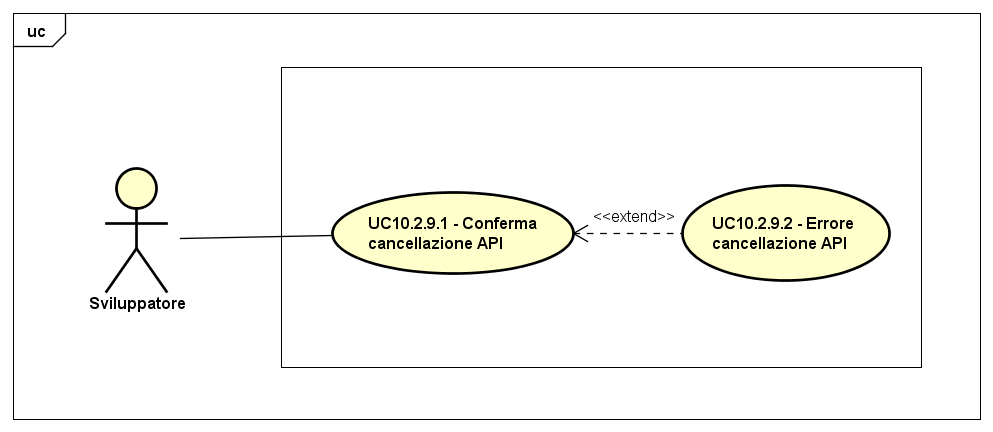
\includegraphics[scale=0.45]{UML/UC10_2_9.png}
	\caption{UC10.2.9: Cancellazione API}
\end{figure}

\begin{minipage}{\linewidth}
	\begin{tabular}{ l | p{11cm}}
		\hline
		\rowcolor{Gray}
		\multicolumn{2}{c}{UC10.2.9 - Cancellazione API} \\
		\hline
		\textbf{Attori} & Sviluppatore \\
		\textbf{Descrizione} & L'attore cancella una API da lui registrata \\
		\textbf{Pre-Condizioni} & L'attore si trova nella schermata relativa alle API da lui registrate \\
		\textbf{Post-Condizioni} & L'attore ha cancellato una API da lui registrata \\
		\textbf{Scenario Principale} & 
		\begin{enumerate*}[label=(\arabic*.),itemjoin={\newline}]
			\item L'attore può confermare la cancellazione di una API da lui registrata (UC10.2.9.1)
		\end{enumerate*}\\
		\textbf{Scenari Alternativi} & 
		\begin{enumerate*}[label=(\arabic*.),itemjoin={\newline}]
			\item L'attore, dopo aver confermato la cancellazione dell'API, può visualizzare un messaggio d'errore informativo (E.g: API con almeno una API key attiva) e la cancellazione non avviene (UC10.2.9.2)
		\end{enumerate*}\\
	\end{tabular}
\end{minipage}

\subparagraph{Caso d'uso UC10.2.9.1: Conferma cancellazione API}
\label{UC10_2_9_1}

\begin{minipage}{\linewidth}
	\begin{tabular}{ l | p{11cm}}
		\hline
		\rowcolor{Gray}
		\multicolumn{2}{c}{UC10.2.9.1 - Conferma cancellazione API} \\
		\hline
		\textbf{Attori} & Sviluppatore \\
		\textbf{Descrizione} & L'attore conferma la cancellazione dell'API, visualizzando un messaggio di successo \\
		\textbf{Pre-Condizioni} & L'attore si trova nella schermata relativa alle API da lui registrate \\
		\textbf{Post-Condizioni} & L'attore ha confermato la cancellazione dell'API, visualizzando un messaggio di successo \\
		\textbf{Scenario Principale} & 
		\begin{enumerate*}[label=(\arabic*.),itemjoin={\newline}]
			\item L'attore può confermare la cancellazione dell'API, visualizzando un messaggio di successo e venendo reindirizzato alla schermata di visualizzazione API registrate (UC10)
		\end{enumerate*}\\
	\end{tabular}
\end{minipage}

\subparagraph{Caso d'uso UC10.2.9.2: Errore cancellazione API}
\label{UC10_2_9_2}

\begin{minipage}{\linewidth}
	\begin{tabular}{ l | p{11cm}}
		\hline
		\rowcolor{Gray}
		\multicolumn{2}{c}{UC10.2.9.2 - Errore cancellazione API} \\
		\hline
		\textbf{Attori} & Sviluppatore \\
		\textbf{Descrizione} & L'attore visualizza un messaggio di errore informativo e la cancellazione dell'API non avviene \\
		\textbf{Pre-Condizioni} & L'attore si trova nella schermata relativa alle API da lui registrate e si è verificato un errore \\
		\textbf{Post-Condizioni} & L'attore ha visualizzato un messaggio di errore informativo \\
		\textbf{Scenario Principale} & 
		\begin{enumerate*}[label=(\arabic*.),itemjoin={\newline}]
			\item L'attore può visualizzare un messaggio di errore informativo e la cancellazione non avviene
		\end{enumerate*}\\
	\end{tabular}
\end{minipage}